\documentclass[UTF8]{ctexart}
\usepackage{subfigure}
\usepackage[graphicx]{realboxes}
\usepackage{listings}
\usepackage{xcolor}
\usepackage{realboxes}

% (1) choose a font that is available as T1
\usepackage{lmodern}
% (2) specify encoding
\usepackage[T1]{fontenc}
% (3) load symbol definitions
\usepackage{textcomp}

\usepackage{fontspec}

\usepackage{hyperref}
\hypersetup{hidelinks,
	colorlinks=true,
	allcolors=black,
	pdfstartview=Fit,
	breaklinks=true}


\definecolor{mygrey}{rgb}{0.945,0.945,0.945}
\definecolor{myred}{rgb}{1, 0.49, 0.63}

\title{K210入门基础}
\author{Liam}
\date{\today}
\lstset{
 basicstyle=\fontspec{Consolas},
 columns=fixed,       
 numbers=left,                                        % 在左侧显示行号
 numberstyle=\tiny\color{gray},                       % 设定行号格式
 frame=none,                                          % 不显示背景边框
 backgroundcolor=\color[RGB]{245,245,244},            % 设定背景颜色
 keywordstyle=\color[RGB]{40,40,255},                 % 设定关键字颜色
 numberstyle=\footnotesize\color{darkgray},           
 commentstyle=\it\color[RGB]{0,96,96},                % 设置代码注释的格式
 stringstyle=\rmfamily\slshape\color[RGB]{128,0,0},   % 设置字符串格式
 showstringspaces=false,                              % 不显示字符串中的空格
 %language=python,                                        % 设置语言
}
%\def\inline{\lstinline[basicstyle=\fontspec{微软雅黑},keywordstyle={}]}

\begin{document}
	\maketitle
	
	\begin{abstract}
		本文将介绍K210的基础部分。
	\end{abstract}
    \section{存储系统}
    \begin{figure}[h]
        \centering
        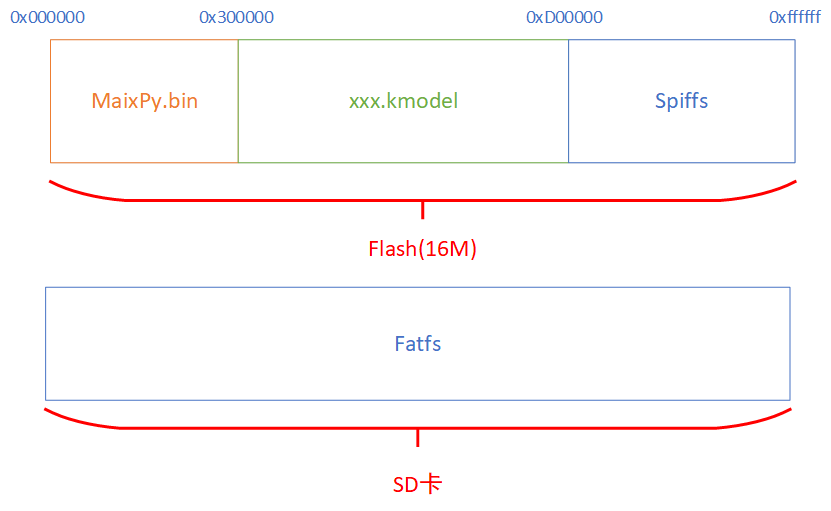
\includegraphics[height=4.5cm,width=9.5cm]{graph/memory.png}
        \label{1}
    \end{figure}
    \subsection*{固件区}
    用来存储MaixPy.py固件,从0x000000开始
    \subsection{模型区}
    但模型区不存放模型
    \subsection{文件系统区}
    该区域交给文件系统管理,文件系统格式为 \textit{spiffs}.不同的文件系统,统一由虚拟文件系统进行管理,提供统一的接口。\underline{3MB}的挂载在\textit{SPIFF},SD卡挂载到\textit{/sd}目录。
    使用示例:
    \lstset{language=python}
    \begin{lstlisting}
        import uos
        print("files:", uos.listdir("/flash"))
        with open("/flash/test.txt", "w") as f:
        f.write("hello text")
        print("files:", uos.listdir("/flash"))
        with open("/flash/test.txt", "r") as f:
        content = f.read()
        print("read:", content)
    \end{lstlisting}
    SD 卡应该满足:
    \begin{enumerate}
        \item 支持 SPI 模式
        \item 分区为 MBR (msdos)
        \item 格式化为 FAT32
    \end{enumerate}
    \subsection{开机自启动脚本}
    系统会在 /flash 或者 /sd(优先) 目录创建 boot.py 文件和main.py, 开机会自动先执行boot.py,然后执行main.py(如果检测到SD卡则执行SD卡里的), 编辑这两个脚本的内容即可实现开机自启,如果在 boot.py 里面写死循环(While True)程序,将会导致 main.py 不能运行(先调用 boot.py 后调用 main.py),重新发送不带死循环的 boot.py 即可解决。
    \begin{itemize}
        \item boot.py 主要用于配置硬件,只配置一次即可。
        \item main.py 可以用于主要的运行的程序。
    \end{itemize}

    \section{功能}
    \subsection{CPU/RAM}
    \begin{itemize}
        \item 复位
        \lstset{language=python}
    \begin{lstlisting}
        import machine
        machine.reset()
    \end{lstlisting}
        \item 主频
        \lstset{language=python}
    \begin{lstlisting}
        from Maix import freq
        freq.set(cpu = 400, kpu = 400)
    \end{lstlisting}
    \end{itemize}

    \subsection{内存管理}
    \begin{itemize}
        \item GC 垃圾回收
        \item 系统\textbf{堆内存}
    \end{itemize}
    GC 内存的总大小是可以设置的, 所以,根据具体的使用情况可以适当修改GC内存大小, 比如:
    \begin{itemize}
        \item 为了加载更大的模型,可以把 GC内存设置小一点
        \item 如果分配新的变量提示内存不足, 可以适当将GC内存设置大一点即可
        \item 如果都不够了, 就要考虑缩减固件大小,或者优化代码了
    \end{itemize}
    \lstset{language=python}
    \begin{lstlisting}
        from Maix import utils
        import machine

        print(utils.gc_heap_size())

        utils.gc_heap_size(1024*1024) # 1MiB
        machine.reset()  
        # reboot after run it
    \end{lstlisting}

    \section{片上外设}
    \subsection{GPIO}
    K210 上有高速GPIO和通用GPIO,每个 IO 可以分配到 FPIOA 上 48 个管脚之一.
    \begin{itemize}
        \item GPIOHS 共 32 个
        \subitem 可配置输入输出信号
        \subitem 每个IO 具有独立中断源
        \subitem 中断支持\textbf{边沿触发}\textbf{电平触发}
        \subitem 可配置上下拉和 \textbf{高阻态}
        \item GPIO 8个
        \subitem 都使用同一个中断源
        \subitem 中断支持\textbf{边沿触发}\textbf{电平触发}
    \end{itemize}

    \subsubsection{构造函数}
    \begin{lstlisting}
        class GPIO(ID,MODE,PULL,VALUE)
    \end{lstlisting}
    \subsubsection{方法}
    参数为空则返回当前状态
    \begin{lstlisting}
        # value
        GPIO.value([value])  
    \end{lstlisting}
    
    GPIO中断模式:
    \begin{enumerate}
        \item GPIO.IRQ\textunderscore RISING
        \item GPIO.TRQ\textunderscore FALLING
        \item GPIO.TRQ\textunderscore BOTH
    \end{enumerate}

   fd

    \begin{lstlisting}
        # irq
        GPIO.irq(CALLBACK_FUNC,TRIGGER_CONDITION,
        GPIO.WAKEUP_NOT_SUPPORT,PRORITY)
    \end{lstlisting}



        关闭中断
    \begin{lstlisting}
        GPIO.disirq()  
    \end{lstlisting}
    \begin{lstlisting}
        GPIO.mode(MODE)
        # GPIO.IN 
        # GPIO.PULL_UP 
        # GPIO.PULL_DOWN
        # GPIO.OUT
    \end{lstlisting}
    
    \subsection{I2C}
    隶属构造函数
    \begin{lstlisting}
class machine.I2C(id,mode=I2C.MODE_MASTER, scl = None,
 sda = None, freq=400000, timeout=1000, addr=0,
 addr_size=7,on_recieve=None, on_transmit=None, 
 on_event=None)
    \end{lstlisting}
    \begin{itemize}
    	\item \colorbox{mygrey}{\color{red}id}: I2C ID, [0~2] (I2C.I2C0~I2C.I2C2) [3~5] (I2C.I2C3~I2C.I2C5, I2C\textunderscore SOFT) 是软模拟 I2C 的编号。
    \end{itemize}
    \subsubsection{方法}
    \begin{itemize}
    	\item \verb|I2C.init(...)|  初始化参数
    	\item \lstinline|i2c.scan()|   扫描从机
    	\item \lstinline|i2c.readfrom(addr, len, stop=True)|       从总线读取数据
    	\item \lstinline|i2c.readfrom_into(addr, buf, stop=True)|   读取数据放在变量中
    	\item \lstinline|i2c.writeto(addr, buf, stop=True)|   发送数据到从机
    	\item \lstinline|i2c.readfrom_mem(addr, memaddr, nbytes, mem_size=8)|    读取从机寄存器
    	\item \lstinline|i2c.readfrom_mem_into(addr, memaddr, buf, mem_size=8)|     读取从机寄存器值到指定变量中
    	\item \lstinline|i2c.writeto_mem(addr, memaddr, buf, mem_size=8)|        写数据到从机寄存器
    	\item \lstinline|i2c.deinit()  /  del i2c| 注销I2C硬件,释放占用的资源,关闭I2C时钟
    \end{itemize}
    \subsection{machine.SPI}
    在 K210 上, SPI 有一下特征:
    \begin{itemize}
        \item 共有 4 个 SPI 设备, 其中 SPI0 、SPI1、 SPI3 只能工作在主机模式下, SPI2 只能工作在从机模式时下, 在 MaixPy 上, SPI3 已经用来连接了 SPI Flash 作为保留硬件资源。
        \item 支持 1/2/4/8 线全双工模式, 在 MaixPy 中, 目前只支持标准(摩托罗拉)4线全双工模式(即 SCK, MOSI, MISO, CS 四个引脚)
        \item 最高传输速率 45M:1/2主频,约 200Mbps
        \item 支持 DMA
        \item 4个可配置任意引脚的硬件片选
    \end{itemize}
    构造函数:
    \begin{lstlisting}
        spi = machine.SPI(id, mode=SPI.MODE_MASTER, baudrate=500000, 
        polarity=0, phase=0, bits=8, firstbit=SPI.MSB, sck, 
        mosi, miso, cs0, cs1, cs2, cs3)
    \end{lstlisting}
    引脚可以使用\colorbox{mygrey}{\color{myred}\lstinline|fm|} 统一管理引脚,从\colorbox{mygrey}{\color{myred}\lstinline|sck|}一下都可以不设置。
    \begin{itemize}
        \item \colorbox{mygrey}{\color{myred}\lstinline|spi.init(id, mode=SPI.MODE_MASTER, baudrate=500000, polarity=0, phase=0, bits=8, firstbit=SPI.MSB, sck, mosi, miso, cs0)|}
        \item \colorbox{mygrey}{\color{myred}\lstinline|spi.readinto(buf, write=0x00, cs=SPI.CS0)|}  
        \item \colorbox{mygrey}{\color{myred}\lstinline|spi.write(buf, cs=SPI.CS0)|}
        \item \colorbox{mygrey}{\color{myred}\lstinline|spi.write(write_buf, read_buf, cs=SPI.CS0)|}
        \item \colorbox{mygrey}{\color{myred}\lstinline|spi.deinit()|}  
    \end{itemize}

    \subsection{machine.PWM}
    隶属构造函数: \colorbox{mygrey}{\lstinline|pwm = machine.PWM(tim, freq, duty, pin, enable=True)|}, 共有3个定时器,最大12路\colorbox{mygrey}{\color{myred}\lstinline|PWM|}
    \par \colorbox{mygrey}{\color{myred}\lstinline|duty|}: 取值为\colorbox{mygrey}{[0,100]}
    \subsubsection{方法}
    \begin{itemize}
        \item \colorbox{mygrey}{\color{myred}\lstinline|pwm.init(tim, freq, duty, pin, enable=True)|}
        \item \colorbox{mygrey}{\color{myred}\lstinline|pwm.freq(freq)|}  获取或者设置频率
        \item \colorbox{mygrey}{\color{myred}\lstinline|pwm.duty(duty)|}
        \item \colorbox{mygrey}{\color{myred}\lstinline|pwm.enable() // pwm.disable()|}
        \item \colorbox{mygrey}{\color{myred}\lstinline|pwm.deinit()|}  
    \end{itemize}

    \subsection{machine.Timer}
    构造函数:
    \par
    \colorbox{mygrey}{\color{myred}\lstinline|tim = machine.Timer(id, channel, 
    mode=Timer.MODE_ONE_SHOT, period=1000, unit=Timer.UNIT_MS, callback=None, arg=None,
     start=True, priority=1, div=0)|}
    \begin{itemize}
        \item  \colorbox{mygrey}{\color{myred}\lstinline|id|}: \colorbox{mygrey}{\color{myred}\lstinline|Timer.TIMER0~TIMER2|}
        \item \colorbox{mygrey}{\color{myred}\lstinline|channel|}: \colorbox{mygrey}{\color{myred}\lstinline|Timer.CHANNEL0~3|}
        \item \colorbox{mygrey}{\color{myred}\lstinline|div|}:  硬件定时器分频器,取值\colorbox{mygrey}{\color{myred}\lstinline|[0,255]|} 定时器时钟频率 = $\frac{clk\_timer}{2^{(div+1)}}$
    \end{itemize}
    \subsubsection{方法}
    \begin{itemize}
        \item \colorbox{mygrey}{\color{myred}\lstinline|tim.init(id, channel, 
        mode=Timer.MODE_ONE_SHOT, period=1000, unit=Timer.UNIT_MS, callback=None, arg=None, 
        start=True, priority=1, div=0)|}
        \item \colorbox{mygrey}{\color{myred}\lstinline|tim.callback(callback)|}
        \item \colorbox{mygrey}{\color{myred}\lstinline|tim.period(period)|}
        \item \colorbox{mygrey}{\color{myred}\lstinline| callback_arg |} 获取设置的传给回调函数的参数。
        \item \colorbox{mygrey}{\color{myred}\lstinline|tim.start()|}
        \item \colorbox{mygrey}{\color{myred}\lstinline|tim.start()|}
        \item \colorbox{mygrey}{\color{myred}\lstinline|tim.restart()|}
        \item \colorbox{mygrey}{\color{myred}\lstinline|tim.deinit()|}
    \end{itemize}
    \subsection{machine.UART}
    k210 一共有3个 uart,每个 uart 可以进行自由的引脚映射。
    \par
    构造函数: \colorbox{mygrey}{\color{myred}\lstinline|uart = machine.UART(uart,baudrate,bits,parity,stop,timeout, read_buf_len)|}
    \begin{itemize}
        \item \colorbox{mygrey}{\color{myred}\lstinline|uart.init()|}
        \item \colorbox{mygrey}{\color{myred}\lstinline|uart.read()|}
        \item \colorbox{mygrey}{\color{myred}\lstinline|uart.readline()|}
        \item \colorbox{mygrey}{\color{myred}\lstinline|uart.write()|}
        \item \colorbox{mygrey}{\color{myred}\lstinline|uart.deinit()|}
    \end{itemize}
    \subsection{machine.WDT}
    MaixPy 的 WDT 看门狗模块,用于在应用程序崩溃且最终进入不可恢复状态时重启系统。一旦开始,当硬件运行期间没有定期进行喂狗(feed)就会在超时后自动复位。
    \begin{lstlisting}
from machine import WDT
wdt0 = WDT(id=1, timeout=4000, callback=on_wdt, context={})
    \end{lstlisting}
    \subsubsection{方法}
    \begin{itemize}
        \item \colorbox{mygrey}{\color{myred}\lstinline|wdt0.feed()|}
        \item \colorbox{mygrey}{\color{myred}\lstinline|wdt0.stop()|}   停止看门狗对象
    \end{itemize}

    \section{Maix库}
    \subsection{FPIOA现场可编程 IO 阵列, Field Programmable Input and Output Array}
    K210 支持每个外设随意映射到任意引脚, 使用 FPIOA 功能来实现。
    \par
    类初始:\colorbox{mygrey}{\color{myred}\lstinline|FPIOA()|}
    \subsubsection{方法}
    \begin{itemize}
        \item \colorbox{mygrey}{\color{myred}\lstinline|fpioa.help()|}
        \item \colorbox{mygrey}{\color{myred}\lstinline|fpioa.set_function(pin,func)|}
        \item \colorbox{mygrey}{\color{myred}\lstinline|get_Pin_num(func)|}
    \end{itemize}
    \section{helper}
    \subsection{fpioa\textunderscore manager}
    fpioa\textunderscore manager:简称fm,该模块用于注册芯片内部功能和引脚,帮助用户管理内部功能和引脚映射关系的功能模块.
    实例:
    \begin{lstlisting}
from fpioa_manager import fm

fm.register(11, fm.fpioa.GPIO0, force=True)
fm.register(12, fm.fpioa.GPIOHS0, force=True)
fm.register(13, fm.fpioa.UART2_TX)
fm.register(14, fm.fpioa.UART2_RX)

# other code

fm.unregister(11)
fm.unregister(12)
fm.unregister(13)
fm.unregister(14)
    \end{lstlisting}
    如果设置 force=False ,则会在 register 发现硬件功能已经被使用了,此时就会弹出异常.
    \par
    有一些引脚已经被注册!!!请查看\url{https://wiki.sipeed.com/soft/maixpy/zh/api_reference/builtin_py/fm.html}
    \begin{itemize}
        \item \colorbox{mygrey}{\color{myred}\lstinline|get_pin_by_function(pin)|}
        \item \colorbox{mygrey}{\color{myred}\lstinline|get_gpio_used() |}
    \end{itemize}
    get\textunderscore gpio\textunderscore used() 返回一个迭代器
    \subsection{Board}
    这是一个 MaixPy 板级配置模块,它可以在用户层统一 Python 代码,从而屏蔽许多硬件的引脚差异。
    \subsection{Micropython Editor}
    MaixPy 固件中集成了文件编辑器 —— pye, 用户可以直接通过串口终端修改板子里面的文件
    \begin{lstlisting}
from pye_mp import pye

pye("/sd/boot.py")
    \end{lstlisting}

    \section{Media资源}
    \subsection{lcd}
    \begin{itemize}
        \item \colorbox{mygrey}{\color{myred}\lstinline|lcd.init(type=1, freq=15000000, color=lcd.BLACK, invert = 0, lcd_type = 0)|}
        \item \colorbox{mygrey}{\color{myred}\lstinline|lcd.deinit()|}
        \item \colorbox{mygrey}{\color{myred}\lstinline|lcd.width()|}
        \item \colorbox{mygrey}{\color{myred}\lstinline|lcd.height()|}
        \item \colorbox{mygrey}{\color{myred}\lstinline|lcd.type()|}
        \item \colorbox{mygrey}{\color{myred}\lstinline|lcd.freq(freq)|}
        \item \colorbox{mygrey}{\color{myred}\lstinline|lcd.get_backlight()|}
        \item \colorbox{mygrey}{\color{myred}\lstinline|lcd.display(image, roi=Auto, oft=(x, y))|}
        \item \colorbox{mygrey}{\color{myred}\lstinline|lcd.clear()|}
        \item \colorbox{mygrey}{\color{myred}\lstinline|lcd.rotation(dir)|}
        \item \colorbox{mygrey}{\color{myred}\lstinline| lcd.bgr_to_rgb(enable)|}
    \end{itemize}

    \subsection{sensor}
    

\end{document}


